\begin{exo}
	On considère un repère orthonormé $\OIJ$.
	\begin{center}
		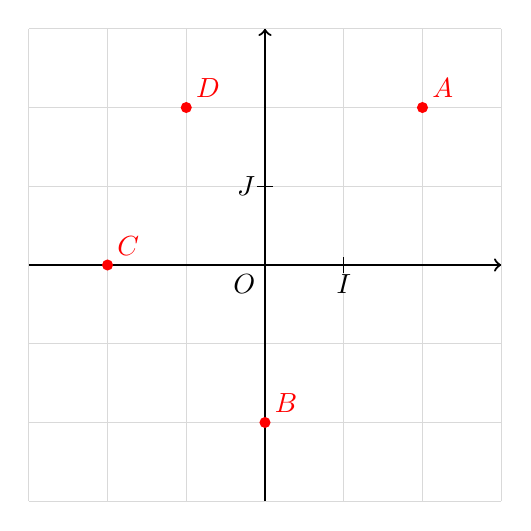
\begin{tikzpicture}
			\draw[step=1cm, gray!30, thin] (-3,-3) grid (3,3);
			\draw[->, thick] (-3,0) -- (3,0);
			\draw[->, thick] (0,-3) -- (0,3);
			\node at (0,0) [below left] {$O$};
			\node at (1,0) [below] {$I$};
			\node at (0,1) [left] {$J$};
			\draw (1,-0.1) -- (1,0.1);
			\draw (-0.1,1) -- (0.1,1);
			\coordinate (A) at (2,2);
			\coordinate (B) at (0,-2);
			\coordinate (C) at (-2,0);
			\coordinate (D) at (-1,2);
			\foreach \p/\name in {A/A, B/B, C/C, D/D} { \fill[red] (\p) circle (2pt); \node[above right, red] at (\p) {$\name$}; }
		\end{tikzpicture}
	\end{center}
	\begin{enumerate}
		\item Déterminer l'ordonnée du point $A$.
		\item Déterminer l'abscisse du point $B$.
		\item Lire les coordonnées des points $C$ et $D$.
	\end{enumerate}
\end{exo}

